\documentclass[a4paper, 12pt]{article}

\usepackage{enumerate}
\usepackage{hyperref}
\hypersetup{
	colorlinks=true,
	linkcolor=blue,
	filecolor=blue,
	urlcolor=blue,
	citecolor=blue,
}
\usepackage{amsmath}
\usepackage{amsthm}
\usepackage{amssymb}
\usepackage[margin=3cm]{geometry}
\usepackage{mathpazo}
\usepackage{url}
\usepackage{subcaption}
\usepackage{tikz}
\usepackage{pgf}
\usepackage{longtable}
\usepackage{multirow}
\usepackage{graphicx}
\usepackage{pgfplots}
\usepackage{cleveref}
\usepackage{amsrefs}
\usepackage{bbm}
\usepackage{csquotes}
\usepackage{wrapfig}
\usepackage{algorithm}
\usepackage{algpseudocode}
\usepackage{mathrsfs}
\usepackage{afterpage}

\numberwithin{equation}{section}
\numberwithin{figure}{section}

\newtheorem{thm}{Theorem}[section]
\newtheorem*{thm*}{Theorem}
\newtheorem*{con*}{Conjecture}
\newtheorem{lem}[thm]{Lemma}
\newtheorem{prop}[thm]{Proposition}
\newtheorem{cor}[thm]{Corollary}
\newtheorem{lemma}[thm]{Lemma}
\newtheorem{conj}[thm]{Conjecture}

\theoremstyle{definition}
\newtheorem{defn}[thm]{Definition}
\newtheorem{remark}[thm]{Remark}
\newtheorem{ex}[thm]{Example}
\newtheorem{quest}[thm]{Question}
\newtheorem{obs}[thm]{Observation}

\renewcommand{\leq}{\leqslant}
\renewcommand{\geq}{\geqslant}
\newcommand{\N}{\mathbb{N}}
\newcommand{\Z}{\mathbb{Z}}
\newcommand{\Q}{\mathbb{Q}}
\newcommand{\R}{\mathbb{R}}
\newcommand{\C}{\mathbb{C}}
\newcommand{\tr}{\mathrm{t}}
\newcommand{\WEEK}[1]{%
\hfill Week #1

\vspace{-1em}

\begin{center}
	\rule{\textwidth}{2pt}
\end{center}
\vspace{0.5em}%
}

\renewcommand{\algorithmicrequire}{\textbf{Input:}}
\renewcommand{\algorithmicensure}{\textbf{Output:}}

\setcounter{tocdepth}{2}

\allowdisplaybreaks

\title{Geometric Foundations of Data Analysis I: \\ Week 4}
\author{Joshua Maglione}
\date{29 September 2025}

\begin{document}

\maketitle
\tableofcontents
\setcounter{section}{2}
\setcounter{subsection}{8}
\setcounter{thm}{3}

\subsection{Coefficient of determination ($R^2$ values)}

The lengths of the differences of the vectors are important and have names: 
\begin{align*} 
	\text{(Sums of Squares Total -- SST)} &: \|Y - \overline{Y} \|^2, \\
	\text{(Sums of Squares Error -- SSE)} &: \| Y - \widehat{Y}\|^2, \\
	\text{(Sums of Squares Regression -- SSR)} &: \| \widehat{Y} - \overline{Y}\|^2 .
\end{align*} 
The value $SST$ measures the \textit{total variability} of the data set. For
example, $\sqrt{SST} = \| Y - \overline{Y} \|$ is the distance from the actual
data $Y$ to the sample mean $Y$. Using the same ideas, we can see that $SSE$
measures the error of our regression and that $SSR$ measures the distance from
our regression to the sample mean. 

\begin{prop}\label{prop:SS-values}
	\[ 
		SST = SSE + SSR. 
	\] 
\end{prop}

\begin{proof}
	Apply Lemma~2.2 and the Pythagorean Theorem:
	\begin{align*} 
		\| Y - \overline{Y} \|^2 &= \| Y - \widehat{Y}\|^2 + \| \widehat{Y} - \overline{Y} \|^2.  \qedhere
	\end{align*} 
\end{proof}

Now we can describe a quantity that measures how good our regression fits the
given data. 

\begin{defn}
	The \textbf{coefficient of determination} (also known as the
	\textbf{$R^2$-value}) is 
	\begin{align*} 
		R^2 &= \dfrac{SSR}{SST} = \dfrac{\|\widehat{Y} - \overline{Y}\|^2}{\| Y - \overline{Y}\|^2} .
	\end{align*} 
\end{defn}

\begin{prop}
	$0\leq R^2 \leq 1$.
\end{prop}

\begin{proof}
	Since each SST and SSR are squares, they are nonnegative. By
	\Cref{prop:SS-values}, we have $0\leq SSR\leq SST$.
\end{proof}

\subsubsection{What do the extremes means?}

The one case where $R^2$ is meaningless is when $SST=0$. This implies both
$SSR=SSE=0$. Moreover, $Y = \overline{Y} = \overline{y} \mathbbm{1}$, where
$\mathbbm{1}$ is the all ones column vector. Hence, every data point $y_i$ is
the same and, therefore, equal to the mean. Let's never return to this case.

We can have $SSR=0$, which is equivalent to $R^2=0$. This implies that $\|
\widehat{Y} - \overline{Y}\|^2= 0$, so that $\widehat{Y} = \overline{Y}$. In
other words, our prediction $\widehat{y}_i$ is just simply the mean. This means
we have not found any relationship between the independent variables and the
dependent variables. 

In the other extreme we have $SSR=SST$, which is equivalent to $R^2=1$. This
implies that $Y = \widehat{Y}$, so the given data lies (exactly) on the surface
given by $y=f(x_1,\dots, x_{p-1})$. That is, the regression function exactly
predicts the data. 

To summarize, when $R^2=0$, we cannot deduce any relationship between the
independent and dependent variables, and when $R^2=1$, we understand completely
the relationship between the independent and dependent variables. Very roughly
speaking, the $R^2$ can be thought of as the ratio of how well the regression
fits the data. 

\subsection{In class exercises pt. III}

\begin{enumerate}
	\item Prove the following.
	\begin{enumerate}
		\item $\| \overline{Y} \|^2 = n\overline{y}$.
		\item $Y \cdot \overline{Y} = \widehat{Y}\cdot \overline{Y} = \| \overline{Y} \|^2$.
		\item $Y\cdot \widehat{Y} = \| \widehat{Y} \|^2$.
	\end{enumerate}
	\item Use (1) to show that 
	\begin{enumerate}
		\item $SST = \|Y\|^2 - \|\overline{Y}\|^2$,
		\item $SSE = \|Y\|^2 - \| \widehat{Y} \|^2$,
		\item $SSR = \| \widehat{Y} \|^2 - \| \overline{Y} \|^2$.
	\end{enumerate}
	\item What are the $R^2$ values for the examples above?
\end{enumerate}


\section{Principal component analysis}

Principal component analysis (PCA) is a power method of analysis that comes
standard in all data science tool kits. With little effort, one can reduce a
complex data set to data that we can more easily see structure. More
specifically, the goal of PCA is to find the ``best'' basis to express the data.
In other words, our initial reference frame may not be the one that best
expresses the structure of our data---PCA is a method to find the ``best''
reference frame.

\subsection{Introducing PCA}

We will start with a toy example, where the analysis is quite simple. Suppose we
have many many data points in $\R^2$ as seen in \Cref{fig:pca-example}.

\begin{figure}[h]
    \centering
    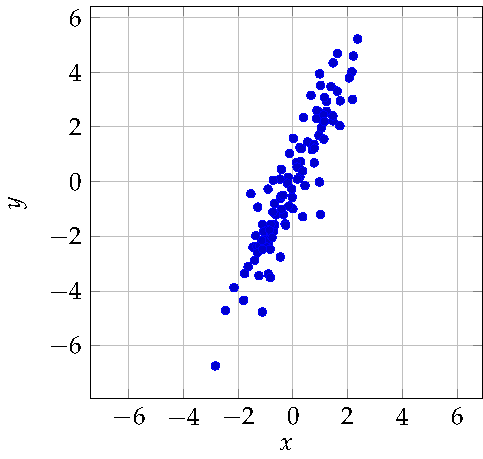
\includegraphics{graphics/pca_example.pdf}
    \caption{Some data in $\mathbb{R}^2$.}
	\label{fig:pca-example}
\end{figure}

Let's assume that our data points live in $\R^m$, so that $m=2$ in
\Cref{fig:pca-example}. Suppose we write those data points in an $m\times n$
matrix $X$. Our current (and default) basis is $\{(1,0, \dots, 0), (0,1, 0,
\dots, 0), \dots, (0,\dots, 0,1)\}$, and we want a basis $\{p_1,p_2, \dots,
p_m\}$ that better reflects the structure of our data. That is, we want an
$m\times m$ matrix $P$, whose rows are the $p_i$, that provides us a better
reference frame. Therefore, we want to transform our data $X$ into a new data
set $Y$ such that 
\[ 
	PX = Y. 
\] 
The columns of $X$ are the ``old'' data, and the columns of $Y$ are the ``new''
data. If the $p_i$ are row vectors and the $x_i$ column vectors, then we want 
\[ 
	PX = \begin{pmatrix} 
		p_1 \\ p_2 \\ \vdots \\ p_m 
	\end{pmatrix} \begin{pmatrix} 
		x_1 & x_2 & \cdots x_n
	\end{pmatrix} = \begin{pmatrix}
		p_1\cdot x_1 & p_1\cdot x_2 & \cdots & p_1\cdot x_n \\
		p_2 \cdot x_1 & p_2 \cdot x_2 & \cdots & p_2 \cdot x_n \\ 
		\vdots & \vdots & \ddots & \vdots \\
		p_m \cdot x_1 & p_m \cdot x_2 & \cdots & p_m \cdot x_n 
	\end{pmatrix}. 
\] 
Thus, if the columns of $Y$ are written $y_i$, we have 
\begin{align}\label{eqn:proj-P}
	y_i &= \begin{pmatrix}
		p_1 \cdot x_i \\ p_2 \cdot x_i \\ \vdots \\ p_m \cdot x_i
	\end{pmatrix}. 
\end{align}

Back to our example from \Cref{fig:pca-example}. We want data with a high
\textit{signal-to-noise} (SNR) ratio as to minimize noise. Assuming our data in
\Cref{fig:pca-example} was collected reasonably well, the direction of largest
variance is the direction of most interesting dynamics. Therefore, the variance
of signal, $\sigma_{\mathrm{s}}^2$, would correspond to the length of the
orange vector in \cref{fig:pca-example2} pointing to the top right, and the
variance of the noise, $\sigma_{\mathrm{n}}^2$, would correspond to the length
of the orange vector pointing to the top left. 

\begin{figure}[h]
    \centering
    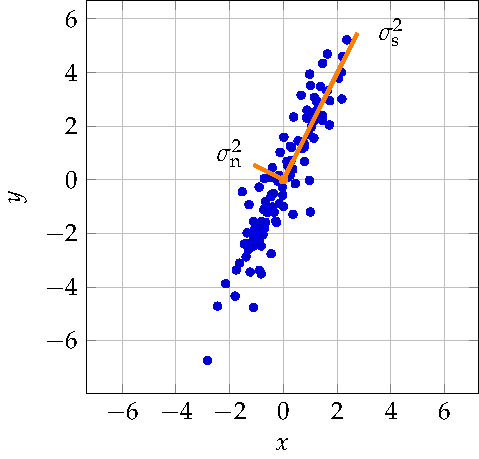
\includegraphics{graphics/pca_example2.pdf}
    \caption{Signal and noise variances represented graphically.}
	\label{fig:pca-example2}
\end{figure}

Note also that in \Cref{fig:pca-example2} knowing the $x$ value gives one a good
approximation for the $y$ value and vice versa. In this case, we might say that
the data has a moderate amount of redundancy, whereas if the data points had a
much higher $R^2$ value to its line of best fit, we would say the data have high
redundancy. (And if the data had a much lower $R^2$ value, we would say the data
have low redundancy.) One of the aims of PCA is to lower redundancy. For the
$2$-dimensional case, this is simple---take the line of best fit, but for
arbitrarily higher dimensions, this is not obvious. 

Suppose we have $n$ measurements of the same kind (like length)
\[ 
	U = \{u_1, u_2, \dots, u_n\} \qquad \text{ and } \qquad V = \{v_1, v_2, \dots, v_n\}
\] 
\textbf{with mean equal to} $\mathbf{0}$. The \textit{variances} are equal to 
\begin{align*} 
	\sigma_U^2 &= \dfrac{1}{n} \sum_{i=1}^n u_i^2, & \sigma_V^2 &= \dfrac{1}{n} \sum_{i=1}^n v_i^2 .
\end{align*} 
The \textit{covariance} between the data sets $U$ and $V$ is 
\begin{align*}
	\sigma_{UV}^2 &= \dfrac{1}{n} \sum_{i=1}^n u_iv_i.
\end{align*}
The covariance measures the degree of the linear relationship between the two
variables. Thus, a large positive value would imply that the data are positively
correlated, and a large negative value would imply negatively correlated. And
$\sigma_{UV}^2= 0$ if and only if the data $U$ and $V$ are uncorrelated.
Moreover the absolute magnitude of the covariance measures the degree of
redundancy. 

If instead we wrote $u = (u_1, u_2, \dots, u_n)$ and $v= (v_1,v_2, \dots, v_n)$
as row vectors, then 
\begin{align}\label{eqn:vec-covar}
	\sigma_{uv}^2 = \dfrac{1}{n} u v^{\tr}. 
\end{align} 
We generalize from two vectors to $m$ vectors. Write 
\begin{align*}
	X = \begin{pmatrix}
		x_1' \\ x_2' \\ \vdots \\ x_m'
	\end{pmatrix}
\end{align*}
where $x_i'$ is a row vector. Note that the rows of $X$ correspond to
measurements of a particular type, and the columns of $X$ correspond to all
measurements of a particular trial. In other words, our data points are the
columns of $X$, and each entry of a data point is a measurement of a particular
type. 

Using \Cref{eqn:vec-covar}, we define the
\textbf{covariance matrix} of $X$ to be 
\begin{align*} 
	C_X &= \dfrac{1}{n} XX^{\tr} .
\end{align*} 

\begin{lem}\label{lem:covariance-properties}
	\hfill 
	\begin{enumerate}
		\item The matrix $C_X$ is symmetric. That is, $C_X = C_X^{\tr}$.
		\item The diagonal entries of $C_X$ are variances.
		\item The off-diagonal entries of $C_X$ are covariances.
	\end{enumerate}
\end{lem}

Recall our goal is to find a new (and better) basis $\{p_1, p_2, \dots, p_m\}$.
Namely, we want an invertible matrix $P$ to turn our data $X$ into a data set
$Y$ where we can better understand the structure. If we could do this on the
level of covariance matrices, then we could pick an ideal covariance matrix, one
where the diagonal entries are large in absolute magnitude and where the
off-diagonal entries are small in absolute magnitude. (Variances being high in
magnitude suggest interesting dynamics, and covariances low in magnitude suggest
low redundancy.) In other words, we would like to find a matrix $P$ such that 
\begin{align}\label{eqn:cov-Y}
	C_Y &= \begin{pmatrix}
		\lambda_1 & 0 & \cdots & 0 \\
		0 & \lambda_2 & \cdots & 0 \\
		\vdots & \vdots & \ddots & \vdots \\
		0 & 0 & \cdots & \lambda_m
	\end{pmatrix},
\end{align}
where $Y = PX$. Typically we have $\lambda_1 \geq \lambda_2 \geq \cdots \geq \lambda_m$.

The main work of PCA is finding such a matrix $P$. We will describe how to
construct such a $P$ later, but let us return to our running example.  

The first principal component is in the direction of the largest variance, and
the second principal component is in the orthogonal direction. So in $\R^2$,
this is quite simple. Although we have not given all the data point explicitly,
the covariance matrix is 
\begin{align*}
	C_X &= \begin{pmatrix}
		1.27 & 2.52 \\
		2.52 & 5.95
	\end{pmatrix}.
\end{align*}
The slope of the line in the direction of the highest variance is 1.98, and it
passes through the point $(0,0)$. By rotating and permuting, we get 
\begin{align*}
	P &= \begin{pmatrix}
		0.40 & 0.92 \\ 0.92 & -0.40 
	\end{pmatrix},
\end{align*}
and the graph of the data $Y = PX$ is seen in \Cref{fig:pca-example3}.

\begin{figure}[h]
    \centering
    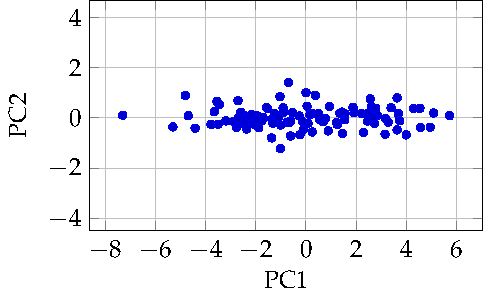
\includegraphics{graphics/pca_example_rotated.pdf}
    \caption{A new basis for our data.}
	\label{fig:pca-example3}
\end{figure}

\begin{remark}
	There is a whole art of scaling data in a pre-processing stage that we will
	not explore in this course. Basically, if one variable ranges between $\pm
	10$ and another $\pm 10^3$, the second variable will bias the process simply
	by its scale. There are many different methods to rescale the data as not to
	lose (too much) information. \textit{Throughout we will assume our data has
	roughly the same scale and not worry about rescaling}, but in practice this
	is an important issue.
\end{remark}














\end{document}